\documentclass[conference]{IEEEtran}
\IEEEoverridecommandlockouts
% The preceding line is only needed to identify funding in the first footnote. If that is unneeded, please comment it out.
\usepackage{cite}
\usepackage{amsmath,amssymb,amsfonts}
\usepackage{algorithmic}
\usepackage{graphicx}
\usepackage{textcomp}
\usepackage{pdfpages}
\usepackage{xcolor}
\usepackage{svg}
\usepackage{float}
\usepackage{hyperref}
\usepackage{url}
\usepackage{graphicx}
\usepackage{dblfloatfix}

\hypersetup{
    colorlinks,
    citecolor=black,
    filecolor=black,
    linkcolor=black,
    urlcolor=black
    pdftitle={EE314 Project Final Report}
}

\makeatletter % changes the catcode of @ to 11
\newcommand{\linebreakand}{%
  \end{@IEEEauthorhalign}
  \hfill\mbox{}\par
  \mbox{}\hfill\begin{@IEEEauthorhalign}
}
\makeatother % changes the catcode of @ back to 12


\def\BibTeX{{\rm B\kern-.05em{\sc i\kern-.025em b}\kern-.08em
    T\kern-.1667em\lower.7ex\hbox{E}\kern-.125emX}}

\begin{document}

\title{EE 314 DIGITAL CIRCUITS LABORATORY 2022-2023 SPRING TERM PROJECT REPORT \\ {\large FPGA IMPLEMANTATION OF A 2D STRATEGY GAME}}

\author{\IEEEauthorblockN{Ahmet Caner Akar}
\IEEEauthorblockA{\textit{Electrical and Electronics Engineering Department} \\
\textit{Middle East Technical University}\\
Ankara, Turkey \\
e244228@metu.edu.tr}
\and
\IEEEauthorblockN{Osama Awad}
\IEEEauthorblockA{\textit{Electrical and Electronics Engineering Department} \\
\textit{Middle East Technical University}\\
Ankara, Turkey \\
e248849@metu.edu.tr}
\and
\linebreakand
\IEEEauthorblockN{İsmail Enes Bülbül}
\IEEEauthorblockA{\textit{Electrical and Electronics Engineering Department} \\
\textit{Middle East Technical University}\\
Ankara, Turkey \\
e244263@metu.edu.tr}
}

\maketitle

\begin{abstract}
This document is about the end-term project of EE314 Digital Circuits Laboratory, implementation of a 2D strategy game by using FPGA.  \\
\end{abstract}

\begin{IEEEkeywords}
FPGA, Verilog HDL, VGA driver, button debouncing, state-machine
\end{IEEEkeywords} 

\section{Introduction}
\section{Project Overview}
\subsection{VGA Module}
\subsection{Button Debouncing and Edge Detector}
In this project, we need to get three inputs, \textbf{logic 1}, \textbf{logic 0} and \textbf{activity}, from the user by using push buttons on the FPGA. However, due to mechanical and physical issues, pushbuttons often generate noisy signals called dirty bounces and these bounces preventing us to properly trigger the program. Thus, to eliminate these undesirable effects, we used debouncing module that makes a noisy pushbutton input signal to ideal input case. \\
\par The working principle of the debouncing module is quite simple. When a button is pressed the timer is going to count the elapsed time up to a predefined threshold parameter. If the timer hits the threshold value, the program concludes that the button reaches its steady-state and it has been pressed. Similarly, when the button is released and the steady state is reached, the program concludes that the button has been released. \\
\par After debouncing button input signal, we designed another module called edge detector to detect the negative and positive edges of the debounced input so that we will use the edge signals directly as button signals in the game controller. \\
\par The button module contains both debouncing module and edge detector module so that the hierarchical design principle is followed throughout the project. Also, both of these modules, are written like a state machine to make it easier to implement condition based and flexible code. The waveform simulation result of the button module in Quartus II is given in Figure 1, below. 
 \begin{figure}[H]
   \centerline{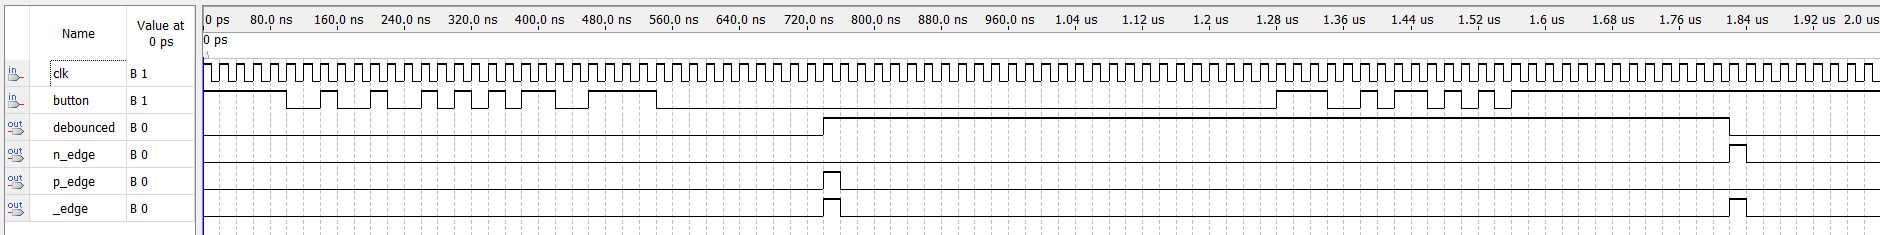
\includegraphics[scale=0.22]{simulation.png}}
    \caption{Button module, waveform simulation result}
\end{figure} 
\subsection{Game Controller}

Example citation \cite{butterworth}
\section{Conclusion}

\bibliographystyle{ieeetr}
\bibliography{refs}
\end{document}
